\section{Theoretical Motivation}
\subsection{Proton Spin Decomposition}
In 1988 the European Muon Collaboration (EMC) found that the proton
spin cannot be attributed solely due to the spin of its
quarks~\cite{EMC_spin}.  Naively it was originally expected the spins
from two valence quarks would cancel each other and the proton's spin
would be due to its third valence quark.  Recent global analysis from
polarized deep inelastic scattering (DIS) at CERN, DESY, and SLAC
surprisingly finds that the quark spin contribution is only about a
quarter of the proton spin~\cite{Spin_globalAnalysis}.  This must mean
that the additional spin of the proton comes from gluon spin and
parton orbital angular momentum.  The total spin structure of the
proton can be summarized as:

\begin{equation}
  \frac{1}{2} = \frac{1}{2}\Delta \Sigma + \Delta \mathrm{G} + \mathrm{L}_{\mathrm{q,g}},
  \label{equ:proton_spin}%
\end{equation}
%
where $\Delta \Sigma$ is the fraction of the proton's spin due to the
quark's spin, $\Delta \mathrm{G}$ is the gluon spin contribution and
$\mathrm{L}_{\mathrm{q,g}}$ is the quark and gluon orbital angular
momentum contribution to the proton spin.

%The spin structure of the proton breaks down this simply in an
%infinite momentum frame called the Breit frame.  In this frame the
%longitudinal which can be approximated experimentally with energies
%about a few GeV.

%\subsection{Transverse Momentum Dependent Parton Distribution Functions}
\subsection{Transverse Momentum Dependent Distributions}

%\begin{figure}[h]
%  \centering 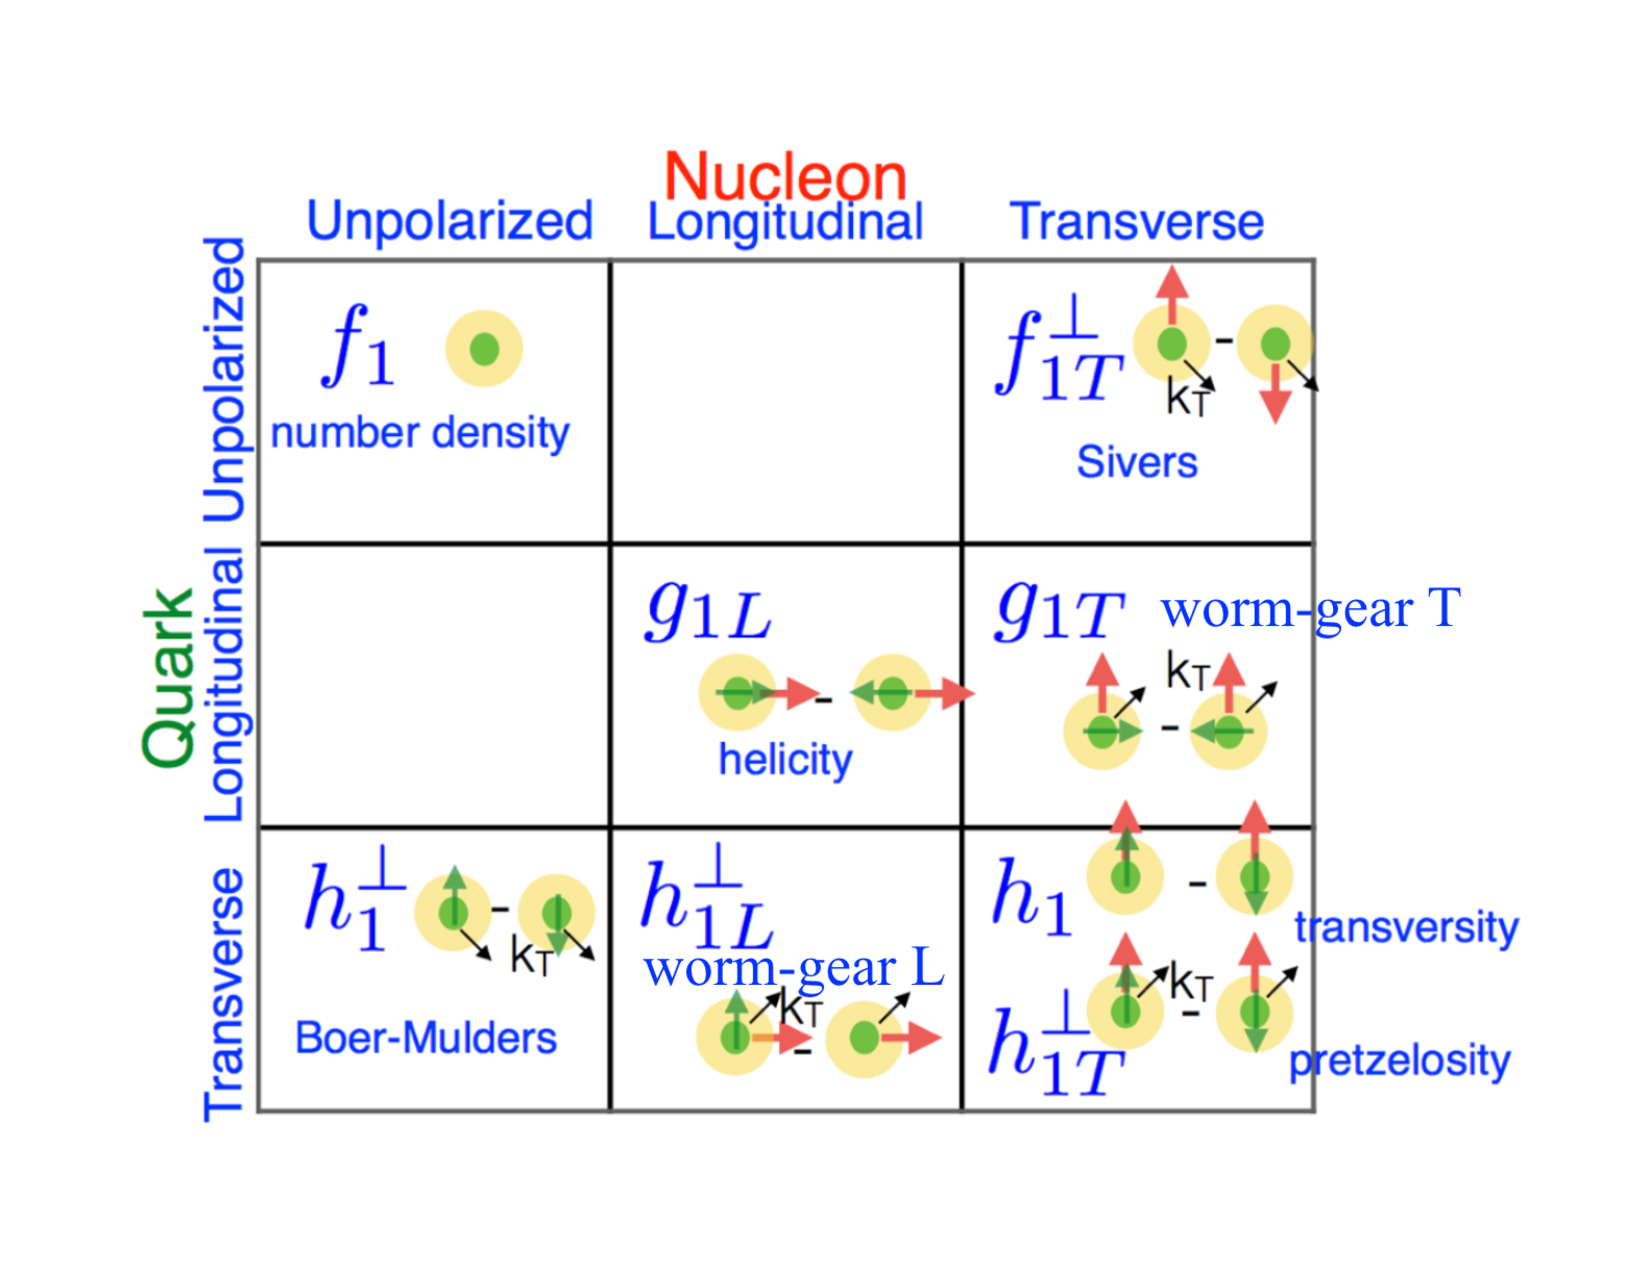
\includegraphics[width=0.6\textwidth]{TMDs}
%  \caption{Transverse momentum dependent distribution functions
%    arranged according to their correlations between the spin of the
%    parent hadron and the spin and/or intrinsic transverse momentum of
%    the parton.}
%  \label{fig:TMDs}
%\end{figure}

\begin{figure}[h]
  \centering
  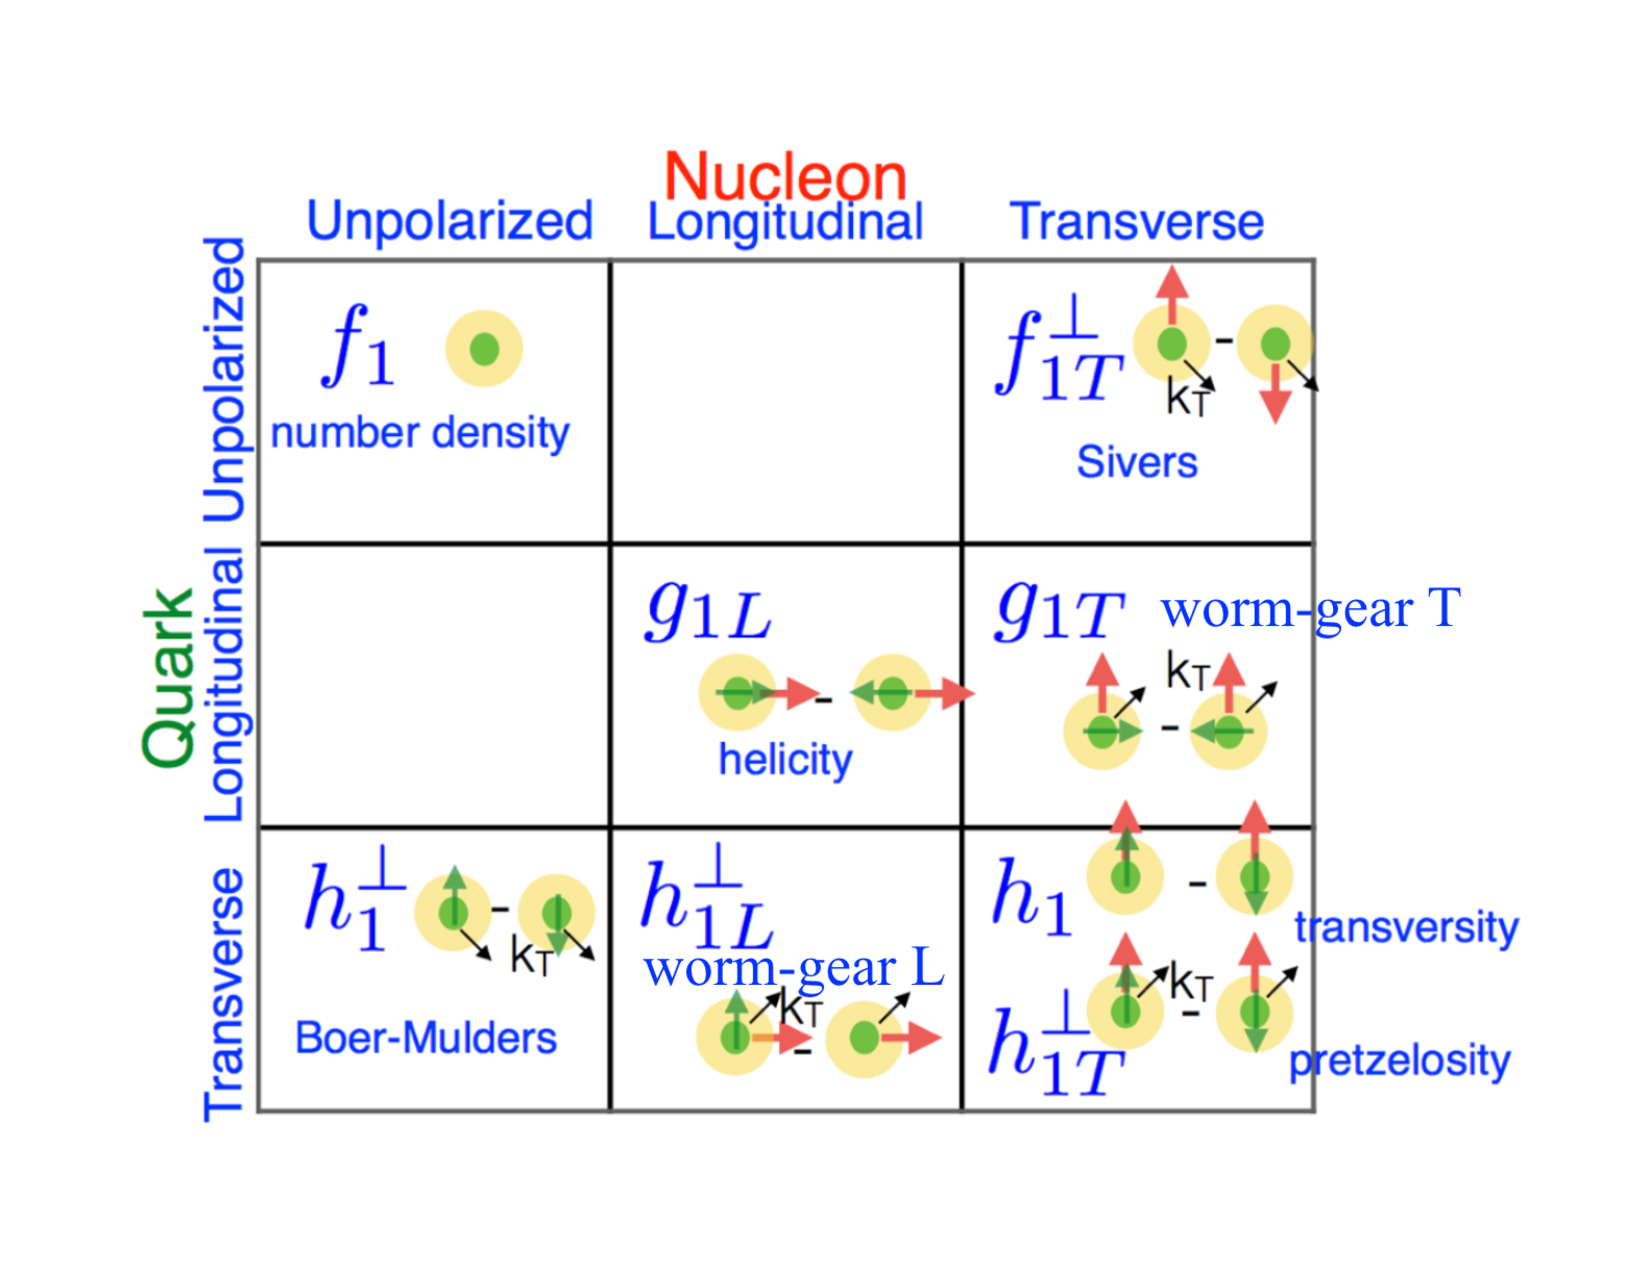
\includegraphics[width=0.5\textwidth,height=0.25\textheight]{TMDs}
  \caption{Transverse momentum dependent distribution functions
    arranged according to their correlations between the spin of the
    parent hadron and the spin and/or intrinsic transverse momentum of
    the parton.}
  \label{fig:TMDs}
\end{figure}

One possible way to describe the orbital angular momentum of quarks in
a hadron is within the framework of transverse momentum dependent
parton distribution functions (TMD).  A systematic treatment of
transverse momentum dependent processes has been developed within the
theory of quantum chromodynamics (QCD) and there are model dependent
connections between TMD functions and orbital angular momentum.
Before the TMD framework, perturbative QCD (pQCD) predicted smaller
transverse momentum effects than what was observed in experiments~\cite{Perdekamp}.
The TMD description improved on pQCD by including soft gluon exchange to account for the transverse momentum of partons which allowed for a better description of
soft non-perturbative contributions to the overall nucleon structure.
The TMD description of the nucleon arises in the cross-section of
hadron scattering and is appropriate when the transverse momentum of
the final state is much less than the invariant mass of the final
state.  When expanding the invariant matrix in powers of
$\frac{1}{\mathrm{Q}^2}$, where $\mathrm{Q}^2$ is the invariant mass
of the exchange force, the leading order contribution called leading
twist, includes eight TMDs to describe a nucleon.  These eight TMDs
are shown in table~\ref{fig:TMDs} arranged according to their
correlation interpretations. \par

%More specifically TMDs are used to
%determine the way partons make up a hadron by describing the
%relationships between the spin of the hadron, the spin of the parton,
%and the transverse momentum of the parton. \par

Two noteworthy TMDs are the Sivers function~\cite{Sivers} and the Boer-Mulders~\cite{Boer-Mulders}
function.  The Sivers function gives a correlation between the
transverse momentum of a parton and the transverse spin of the parent
hadron.  Although there is currently no quark orbital angular momentum
observable, a bound quark with transverse momentum does not depart
from the proton and therefore the Sivers function is thought to be
related to parton orbital angular momentum in that measuring a
non-zero Sivers function indicates a quark has orbital angular
momentum.  The Boer-Mulders function gives a correlation between the
transverse momentum of the parton and the transverse spin of the same
parton.  The Sivers and the Boer-Mulders distributions are interesting
because they are theorized to be independent of any physical processes
up to a sign change~\cite{collins_2002}.  It is theorized that the Sivers and Boer-Mulders
functions change sign between the semi-inclusive deep inelastic
scattering (SIDIS) process and the Drell-Yan process as in
equations~\ref{equ:SivBM}.  This semi-universality arises because the
Sivers and Boer-Mulders functions are time reversal odd and in the
Drell-Yan process there are only initial state gluons while in SIDIS
there are only final state gluons.  Comparing the Sivers function or
the Boer-Mulders function between the SIDIS and the Drell-Yan
processes is therefore a fundamental test of the underlying TMD and QCD theory.



\begin{multicols}{2}
  \begin{equation}
    \begin{aligned}
      & \text{Sivers} \\
      & f^{\perp}_{1T}\mid _{Drell-Yan} = -f^{\perp}_{1T}\mid _{SIDIS} 
    \end{aligned}
  \end{equation}\break
  \begin{equation}
    \begin{aligned}
      & \text{Boer-Mulders} \\
      & h^{\perp}_{1}\mid _{Drell-Yan} = -h^{\perp}_{1}\mid _{SIDIS}
    \end{aligned}
  \end{equation}\break
  \label{equ:SivBM}%
\end{multicols}

%\begin{multicols}{2}
%  \begin{equation}
%    \text{Sivers} 
%    f^{\perp}_{1T}\mid _{Drell-Yan} = -f^{\perp}_{1T}\mid _{SIDIS} 
%    \label{equ:Sivers}
%    %\caption{The Sivers function.}
%  \end{equation}\break
%  \begin{equation}
%    h^{\perp}_{1}\mid _{Drell-Yan} = -h^{\perp}_{1}\mid _{SIDIS}
%    %\caption{Boer-Mulders function.}
%  \end{equation}\break
%  \label{equ:SivBM}%
%\end{multicols}



\subsection{The Drell-Yan Process}

The Drell-Yan process was proposed in 1970 to describe the
cross-section where the final state results in two oppositely charged
leptons \cite{DY_process}.  The process involves the annihilation of a
quark and an anti-quark into a virtual photon, Z-boson or W-boson,
which then decays into a lepton and an anti-lepton pair.  The Drell-Yan reaction for a polarized target is given in
equation~\ref{equ:ComDY} and the correspond Feynman diagram is given
in figure~\ref{fig:fey_DY}.
%
\begin{equation}
  H_a(P_a) + H_b(P_b, S_b) \rightarrow \gamma ^*(q) + X \rightarrow
  l^-(l) + l^+(l') + X
  \label{equ:ComDY}
\end{equation}
%
\begin{figure}[h]
  \includegraphics[width=0.5\textwidth,center]{feyDY}
  \caption{}{The Drell-Yan Feynman diagram for a polarized
    target where $\bar{u}$ and $u$ are the annihilating quarks
    and the invariant mass is low enough so only an electro-magnetic
    reaction can occur.}
  \label{fig:fey_DY}
\end{figure}
%
Here $\mathrm{H}_{\mathrm{a(b)}}(\mathrm{P}_{\mathrm{a(b)}}, \mathrm{S}_{\mathrm{b}})$ represents the initial state hadron as
a function of the 4-momentum and 4-spin vectors, $\gamma^{*}$ is a virtual photon,
$l^{+(-)}$ are the measured final state leptons and $X$ represents
what is not measured.  In all cases subscript a (b) will refer to the
beam (target).  Specifically the leptons studied at COMPASS were final
state muons.  This is because muons have a long range which makes
them easier to detect and study experimentally. Kinematic variables
of interest in the Drell-Yan process are as shown in
equations~\ref{equ:s}-~\ref{equ:M2}.

\begin{subequations}
  \begin{align}
    &s = (P_a + P_b)^2 & \text{Center of momentum energy
      squared.}\label{equ:s}\\ &x_{a(b)} = \frac{q^2}{P_{a(b)} \cdot
      q} & \text{x-Bjorken, parton longitudinal momentum fraction.}
    \\ &x_f = x_a - x_b & \text{x-Feynman variable.}\\ &M^2 = q^2 =
    sx_ax_b & \text{Invariant mass of the virtual
      photon.}\label{equ:M2}
  \end{align}
  \label{equ:DYkin}
\end{subequations}

One of the defining characteristics of the Drell-Yan process is a
steep falloff of the cross-section as a function of the invariant mass.
Above 4~$\frac{\mathrm{GeV}}{\mathrm{c}^2}$ the cross-section is of the order of
nano-barns.  This makes the Drell-Yan process experimentally
challenging because the beam intensity must therefore be quite high
while at the same time having the background well suppressed.  From
the theoretical point of view, however, the Drell-Yan process is
considered to be cleaner than other processes such as SIDIS.  This is
due to the fact that only initial state soft, non-perturbative terms
describe the process.  There are no final state quarks leading to the
need for non-perturbative fragmentation functions.  The only soft
terms come from the parton distribution functions (PDF) of the
incoming hadrons. \par

One of the most interesting features of the Drell-Yan process is its
ability to access TMDs experimentally.
Through the Drell-Yan process with the transversely polarized target
and an unpolarized pion beam, as in the 2015 COMPASS data taking, there is
the possibility to extract the Sivers amplitude, the Boer-Mulders
amplitude, the prezelosity amplitude and the transversity amplitude \cite{DYxSection}.  The
leading order Drell-Yan cross-section for an unpolarized beam on a
transversely polarized target is given in equation~\ref{DY-xsection},

\begin{dmath}
\frac{d\sigma}{d^4qd\Omega} = \frac{\alpha^2_{em}}{Fq^2}\hat{\sigma}_U
\Bigg \{ \Big(1 + D_{[\sin^2(\theta)]}A_U^{\cos(2\phi)}\cos(2\phi)\Big )
+ \| S_T \| \Big [ A_T^{\sin(\phi_S)}\sin(\phi_S) +
  D_{[\sin^2(\theta)]}\Big
  (A_T^{\sin(2\phi+\phi_S)}\sin(2\phi+\phi_S)+A_T^{\sin(2\phi-\phi_S)}\sin(2\phi-\phi_S)\Big
  ) \Big ] \Bigg \},
\label{DY-xsection}%
\end{dmath}
%
where $F$ is the flux, $D_{[f(\theta)]}$ is a depolarization factor,
$\| S_t \|$ is the transverse polarization percentage and $\hat{\sigma}_U$
is the spin-independent Drell-Yan cross-section.\par

To describe the different angles used in the Drell-Yan cross-section,
the description of the transversely polarized Drell-Yan process is
done in a target frame and a center of momentum frame called the
Collins-Sopers frame ~\cite{CollinSoperFrame}.  The target coordinate
system, figure~\ref{fig:CSframe}, is the frame where the beam is along
the z-axis and the virtual photon is along the x-axis.  The phi
Sivers, $\phi_S$, angle is defined in the target frame.  The
Collins-Sopers coordinate system, figure~\ref{fig:CSframe}, comes from
boosting out of the target frame along the z-axis and then boosting
along the x-axis.  The Collins-Sopers frame gives the additional
$\phi$ and $\theta$ angles used in the description of the
cross-section \cite{CollinSoperFrame}.

\begin{figure}[h]
  \centering
  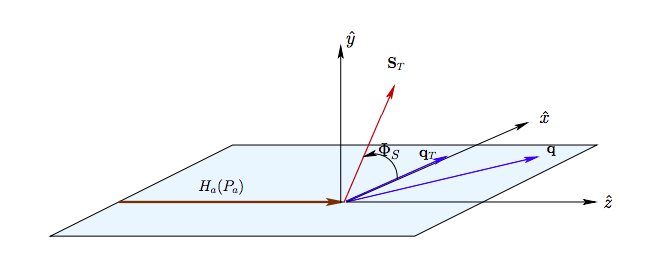
\includegraphics[width=0.47\textwidth]{TargFrame}
  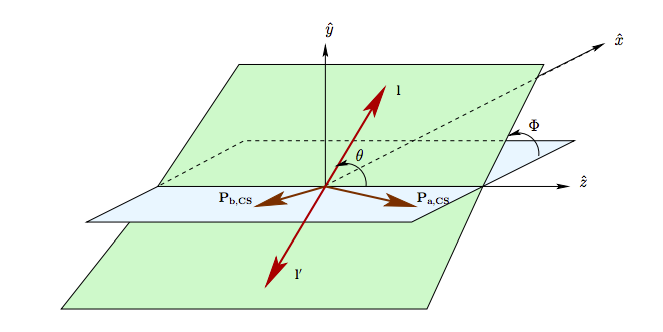
\includegraphics[width=0.47\textwidth]{CSframe}
    \caption{In the left panel the target frame has the z-coordinate
      aligned with the incoming beam and the x-coordinate aligned with
      the virtual photon.  In the right panel the Collins-Soper frame
      is a center of momentum frame which can be reached from the
      target frame by a boost along the z-direction followed by boost
      in the x-direction.  The Collins-Soper frame is defined by
      having the z-axis bisect the momentum components of P$_a$ and
      -P$_b$.}
    \label{fig:CSframe}%
\end{figure}
    
Under the factorization theorem when the virtual photon invariant
mass, $q^2$, is much greater than its transverse momentum, $q_T$, the
cross-section amplitudes give a convolution of PDFs or TMDs of the
beam and the target.  An example of this relation for the Sivers
function is shown in equations~\ref{equ:Corr}-~\ref{equ:AT}.
%
\begin{subequations}
  \begin{align}
    \begin{split}
      C[w(k_{aT},k_{bT})f_a\bar{f}_b)] = \frac{1}{N_c}\sum_q e_q^2\int
      d^2k_{aT}d^2k_{bT}\delta^{(2)}(q_T - k_{aT}-k_{bT})w(k_{aT},
      k_{bT})\times\\ \Big [ f^q_a(x_a, k^2_{aT})f^{\bar q}_2(x_b,
        k^2_{bT}) + f^{\bar q}_1(x_a, k^2_{aT})f^q_2(x_b, k^2_{bT})
        \Big ] \quad \text{Correlation function.}\label{equ:Corr}
      \end{split}\\
    & F^1_U = C[f_a\bar{f}_b] \Repeat{11}{\qquad} \text{$F^1_U$
      definition. }\\ & A_T^{\sin(\phi_S)} = \frac{C[h \cdot k_{bT}f_a
        \bar{f}^{\perp}_{1T}]}{M_b F^1_U} \Repeat{8}{\qquad}
    \text{Sivers amplitude.}\label{equ:AT}
  \end{align}
  \label{equ:SivCorr}
\end{subequations}
%
This means one can access the Sivers function,
$\bar{f}^{\perp}_{1T}$, for the proton through measuring the Sivers
amplitude, $A_T^{\sin(\phi_S)}$.  In a similar manner, the amplitude
$A_T^{\sin(2\phi+\phi_S)}$ is sensitive to the prezelosity function,
the amplitude $A_T^{\sin(2\phi-\phi_S)}$ is sensitive to the
transversity function and the amplitude $A_U^{\cos(2\phi)}$ is
sensitive to the Boer-Mulders function.  Therefore the Sivers,
prezelosity and transversity amplitudes can be extracted from
single-spin asymmetries, while the Boer-Mulders amplitude can be
extracted from spin-independent Drell-Yan data. \par

